% John L. Godlee (johngodlee@gmail.com)

\documentclass[a4paper, 11pt]{article}
%
\usepackage{amsmath}   % Better maths and more symbols
%
\usepackage{siunitx}
%
\usepackage{geometry}  % Set margins
	\geometry{left=2.2cm,
		right=2.2cm,
		top=2.2cm,
		bottom=2cm}
\parskip 0.5cm
\setlength{\parindent}{0.5cm}
%\twocolumn
%
\usepackage{pdflscape} % Allow landscape pages nested in pdf
%
\usepackage{graphics}  % Insert images easily
\usepackage{graphicx}
\graphicspath{ {img/} }
\usepackage{float}  % Fancy graphics placement [H] [H!] arguments
\usepackage{subfig}
%
\usepackage{caption}
%
\usepackage{enumerate}
%
\usepackage{natbib}    % Bibliography management - Use author/date citations
\bibliographystyle{agsmnourl}  % Use my custom agsm bibliography template which never includes URLs in articles
\usepackage{url}
\usepackage{cite}
%
\usepackage{lineno}
\linenumbers
%
\usepackage{eurosym}
\usepackage{textcomp}
\newcommand{\textapprox}{\raisebox{0.5ex}{\texttildelow}}
%
\usepackage{color} 
\newcommand{\todo}[1]{\textcolor{red}{#1}}   % \todo{NOTE TO SELF WRITTEN IN RED}

\title{Changes in forest structure along an elevational gradient in the Peruvian Andes cause species-specific stress responses in tree seedlings}
\author{John L. Godlee}

%--------------------------------------------------------------
\begin{document}
%--------------------------------------------------------------

\maketitle{}

\begin{abstract}
\noindent

\begin{itemize}
\item{We assessed the contribution of biotic competition factors to limiting elevational range shifts of tree species along an Amazon to Andes elevational gradient, focussing on tree seedlings as a key demographic bottleneck for future recruitment.}
\item{Photocynthetic capacity measured using chlorophyll fluorescence estimated photosynthetic stress experienced by naturally occurring seedlings of seven tree species spanning the elevational gradient. Physiognomic plant traits were also measured to assess the degree of local acclimatory response to elevationally dependent environmental factors.}
\item{We used linear mixed effects models to compare the effect sizes of individual biotic competition fixed effects against that of elevation. A matrix of multiple fixed effect mixed effects models were compared statistically to ascertain the best combination of predictors affecting seedling growth and stress metrics.}
\item{}
\end{itemize}

4 bullet points (1) research conducted + rationale, (2) central methods, (3) key results, (4) main conclusions including key points of discussion. 
	
\end{abstract}


\section{Introduction}
Rapid anthropogenic climate change is causing many species, across a wide range of taxa, to shift their distributions in space \citep{Hughes2000, Parmesan2006, Chen2011}. The primary forces driving this are an increase in temperature and changes in precipitation regime \citep{Corlett2013, McCain2011}. \citet{Chen2011} estimates that across a range of taxonomic groups, species are experiencing mean latitudinal and altitudinal migration rates of 17.6 $\pm$ 2.9 km and 12.2 $\pm$ 1.8 m per decade, respectively. Previous studies have suggested that the ability of tree species to respond to changes in mean annual temperature and precipitation regime will be important in determining species success over the coming century \citep{Colwell2008, Chen2011, Feeley2012}. Species responses may occur either in the form of adaptation, \textit{i.e.} changes in phenology, physiology and morphology, or through range shifts over space \citep{Bellard2012}. Range shifts of tree species have been observed in many studies across the world, particularly in temperate, sub-arctic and mountainous regions \citep{} where temperature change is the most extreme \citep{}. The number of studies documenting adaptational responses are fewer, potentially indicating that climate change is occurring so rapidly as to prevent effective adaptational responses \citep{}. Range shift rates vary between tree species. This has the potential to create new species assemblages as species ranges overlap more or less as they shift, with consequences for ecosystem functionality as novel forest assemblages are created. Predicting range shifts across space has become an active field of research, (see \citealt{Bellard2012} and references therein). Understanding the drivers of range shifts and their variation between species can aid in the identification of species assemblages at risk of extinction and can inform conservation strategies to mitigate the effects of climate change on biodiversity and ecosystem functionality \citep{}.

The majority of species distribution models used to predict species range shifts as a conservation tool have used bioclimatic envelopes to constrain species' ranges \citep{Pearson2003, Sinclair2010}. Bioclimatic envelopes are constructed by correlating current species range extent with observed environmental conditions within those boundaries, then projecting spatially explicit climate trends into the future under different climate change scenarios to predict how species range boundaries will adjust in response (e.g. \citealt{Berry2002, Peterson2002, Thuiller2005, Araujo2006}). These models have been criticised often for being overly simplistic, especially when applied at the local scale \citep{}, where other factors that have not been considered by the bioclimatic envelope model become important limiting factors for a species. Such factors include unmeasured environmental variables, physical factors such as topography, and biotic interactions with other species \citep{Davis1998, Putten2010, Ettinger2011}. 

When range shifts in a rapidly changing climate are driven by a single environmental variable like mean annual temperature, it is possible that a species will move into an area that is sub-optimal in other ways than those predicted by the model if range shifts outstrip acclimatory/adaptive potential \citep{}. Range shifts into sub-optimal habitats may lead to reductions in local species abundance and/or richness \citep{Colwell2008}, changes in community composition \citep{}, ecosystem functioning \citep{Bellard2012}, and ecosystem service provision that are not predicted by bioclimatic envelope models \citep{Dobson2011, Isbell2011}. In order to accurately predict range shifts and their consequences for future ecosystem assembly, it is important that predictive range models be expanded to include variables which describe habitat as well as climate, and consider ecosystem level effects rather than simply species level effects \citep{}.

For sessile taxa such as trees, range shifts occur as a result of differential recruitment and mortality over space, at the leading and trailing edges of their range \citep{}. 
In communities of long-lived tree species, the forest ecosystem may not shift in equilibrium with the climate as trees are resilient to gradual changes in climate, developing large root systems and below-ground water and nutrient reserves to buffer against stressful conditions; adult trees may persist where more sensitive seedlings perish \citep{}. Forest trees, particularly those in moist tropical forests, often experience high levels of mortality during the seedling recruitment stage, creating a demographic bottleneck \citep{Coomes2000}. Many seedlings perish due to suboptimal shade regimes created by the arrangement of adult trees creating canopy above them \citep{}. The seedlings of many tropical tree species are highly adapted to shade \citep{}, meaning that if a seedling germinates in an open space, mortality by UV-B and heat damage to photosynthetic machinery is quite probable \citep{}. Seedlings may also compete with adult trees for nutrients \citep{}, although there is some separation between seedling and adult tree rooting depths for most species \citep{}, especially for the largest trees \citep{}. This mortality bottleneck provides a limiting factor to the success of tropical forest tree species experiencing range shifts. If seedlings germinate in areas that are only sparsely shaded but are within temperature boundaries, damage may occur leading to loss of photosynthetic capacity \citep{}, reducing growth rates and occasionally resulting in seedling mortality \citep{}.  

In montane cloud forests, elevational range shifts are occurring more rapidly than in other areas \citep{}. As mean annual temperatures rise, plant species are figuratively pushed up-slope, with higher recruitment at the upslope edge of their range and higher mortality at the downslope edge of their range \citep{}. Particularly in the tropics, as altitude increases, UV-B concentration increases, with many species found at high altitudes \citep{} having specific adaptations to avoid UV-B damage to photosynthetic machinery, such as vertically stacked palisade mesophyll cells and thick cuticles to reduce UV-B absorption, and generally smaller thicker leaves \citep{}. Species found at low altitudes however, are less adapted to high UV-B environments, instead having adaptations to make the most of the diminished light levels found under thick tree canopy, particularly during the seedling growth stage \citep{}. Montane forest physical structure also varies with elevation. Lowland forests often have lower tree density, with relatively few young trees in the light-deprived understorey, but a higher canopy cover due to adult trees being larger. Plant ground cover is generally greater at higher altitudes, with many epiphytic and ground-level herbaceous species. It therefore follows that as lowland species move upslope in response to increasing temperature, they may experience increased levels of damaging UV-B radiation as they recruit into areas of forest with thinner canopies. This may lead to species' ranges narrowing form the bottom up, with increased mortality due to temperature at the bottom of the elevational range, but without increased recruitment at the top end of the elevational range due to increased mortality via UV-B exposure.

In this study, we investigated the effects of variation in adult tree canopy structure and size distribution on seedling growth form and photosynthetic stress, across an elevational gradient in the Peruvian Andes, spanning lowland wet forest and montane cloud forest. Our aim was to assess the role of biotic effects from the existing forest structure on the potential growth of tree seedlings, in order to increase our knowledge of the dynamics of montane cloud forest tree species elevational range shifts. We tested three hypotheses: 1) Within a species, seedlings growing at higher elevations would experience higher levels of photosynthetic stress than those at lower elevations, 2) Species would differ in their degree of acclimation to variation in adult tree canopy structure and size distribution, 3) A combination of biotic and abiotic explanatory variables would best explain variation in seedling physiognomic and physiological traits across their elevational range.  

\section{Materials and Methods}
\subsection{Study Site}
Data collection was conducted across 10 permanent 1 ha forest plots in the Kos\~{n}ipata Valley of Man\'{u} National Park, Peru (-13\textdegree N, -71\textdegree W, Figure \ref{fig:sites}, Table \ref{table:sitechar}). The Kos\~{n}ipata Valley has been identified as a migration corridor for lowland species to migrate to higher elevations in response to temperature increase \citep{Feeley2011} and so is an appropriate location to study range shift drivers. Plots are situated between 400 and 3200 m.a.s.l. along this migration corridor (Table \ref{table:sitechar}, Figure \ref{fig:range_plot}). The plots form part of a larger plot network established by the Andes Biodiversity and Ecosystem Research Group (ABERG) in 2003 \citep{Malhi2010, Girardin2014}, and are located within the ``Tropical Andes'' biodiversity hotspot identified in \citet{Myers2000}. The plots used in this study contain 719 tree species, and the valley as a whole contains an estimated 1167 tree species \citep{}.

\begin{figure}[H]
\includegraphics[width=\textwidth]{sites}
\centering
\caption{Maps showing the location of the study area and plot locations. (A) The site location within Peru with elevation shading, showing the proximity to Man\'{u} National Park (white area). (B) The location of the 1 ha plots within the Kos\~{n}ipata Valley. (C) An enlargement of the Trocha Union and San Pedro plot groups. Red crosses indicate plot location, white lines in maps (B) and (C) indicate roads, text labels in (B) and (C) are plot codes, dark green areas in (B) and (C) denote the bounds of Man\'{u} National Park.}
\label{fig:sites}
\end{figure}

\subsection{Study species} 
We chose seven tree species for comparison from a total of 719 identified species within the 10 study plots. Species were selected according to their contrasting ranges (Figure \ref{fig:range_plot}), differences in genus migratory pattern \citep{Feeley2011}, and because each species is dominant across it's range in the Kos\~{n}ipata Valley (ABERG, unpublished data, \todo{Appendix VI}). Seedlings of \textit{Myrcia spp.} are difficult to reliably identify to species in the field due to similar morphology and were thus sampled as a composite of three potential species: \textit{Myrcia splendens}, \textit{M. fallax}, and \textit{M. rostrata}, the only \textit{Myrcia} species known to be present in our plots from ABERG censuses. They are referred to as \textit{Myrcia spp.} from here onwards. 

% Despite having no quantitative range shift prediction information, \textit{Iriartea deltoidea} and \textit{Dictyocaryum lamarckianum} were included in order to observe potential differences in response between monocot and dicot species, as both are monocots. Both \textit{I. deltoidea} and \textit{D. lamarckianum} are large-seeded palm species, as such, they are expected to be migrating upslope, similar to other large-seeded palms \citep{Hillyer2010}.

\begin{figure}[H]
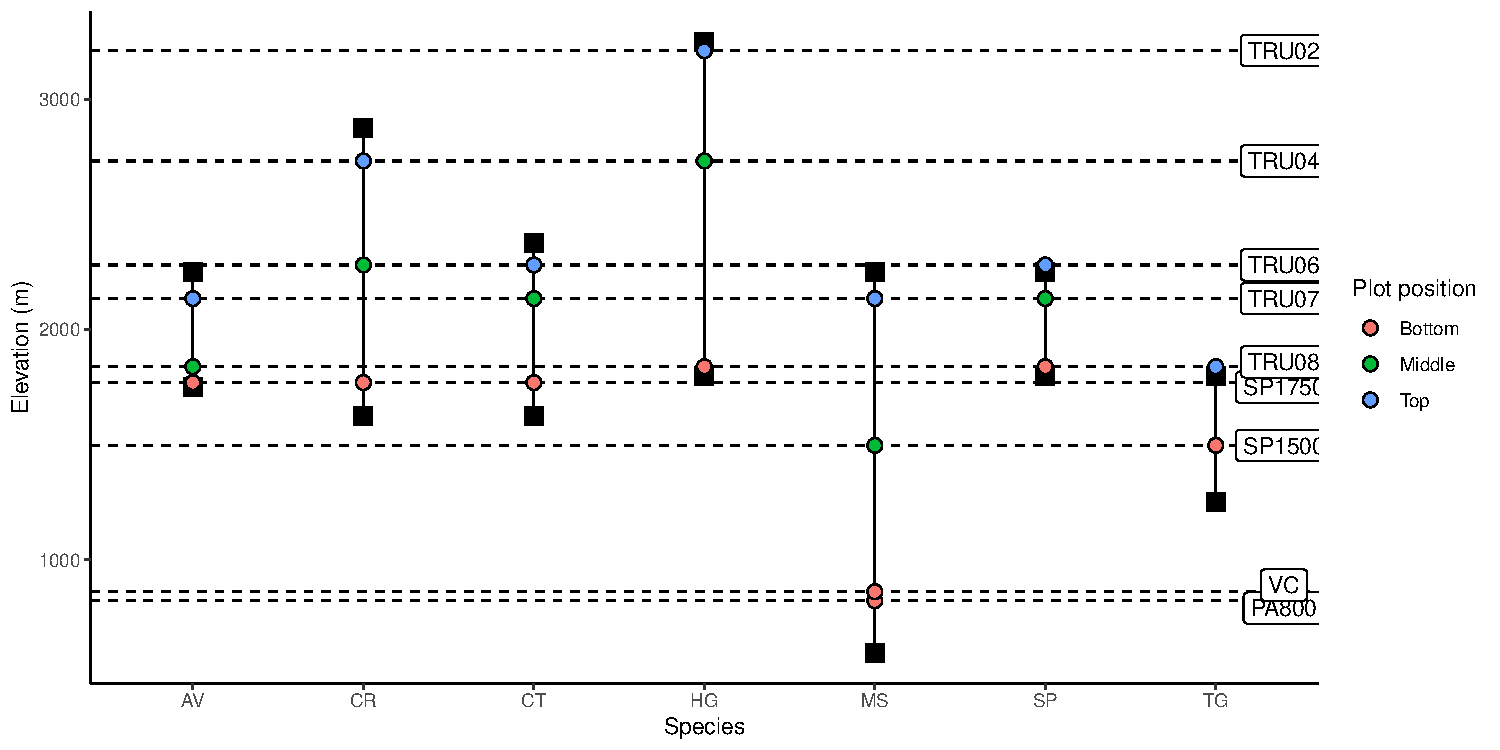
\includegraphics[width=\textwidth]{ranges}
\centering
\caption{Elevation of study plots for each species (coloured points) with the upper and lower range extents for each species (black squares). Plot elevations are marked as dashed lines.}
\label{fig:ranges_ggplot}
\end{figure}


% Table created by stargazer v.5.2.2 by Marek Hlavac, Harvard University. E-mail: hlavac at fas.harvard.edu
% Date and time: Mon, Oct 21, 2019 - 19:13:07
\begin{table}[!htbp] \centering 
  \caption{The site names at which tree seedlings were sampled for each species, with the number of seedlings successfully sampled per site for each species.} 
  \label{species_elevcode_tally} 
\begin{tabular}{@{\extracolsep{5pt}} llr@{\hspace{0.2\tabcolsep}}lr@{\hspace{0.2\tabcolsep}}lr@{\hspace{0.2\tabcolsep}}l} 
\\[-1.8ex]\hline 
\hline \\[-1.8ex] 
{Species code} & {Species} & \multicolumn{2}{c}{Bottom} & \multicolumn{2}{c}{Middle} & \multicolumn{2}{c}{Top} \\
\hline \\[-1.8ex] 
AV & \textit{Alzatea verticillata} & SP2 & =7 & TU8 & =5 & TU7 & =6 \\ 
CR & \textit{Clethra revoluta} & SP2 & =7 & NA & & TU4 & =8 \\ 
CT & \textit{Clusia thurifera} & SP2 & =9 & TU7 & =9 & NA & \\ 
HG & \textit{Hedyosmum goudotianum} & TU8 & =10 & TU4 & =10 & TU2 & =11 \\ 
MS & \textit{Myrcia} spp. & PA2 & =10 & SP1 & =8 & TU7 & =10 \\ 
SP & \textit{Schefflera patula} & TU8 & =9 & TU7 & =12 & NA & \\ 
TG & \textit{Tapirira guianensis} & SP1 & =10 & NA & & TU8 & =10 \\ 
\hline \\[-1.8ex] 
\end{tabular} 
\end{table} 


\begin{figure}[H]
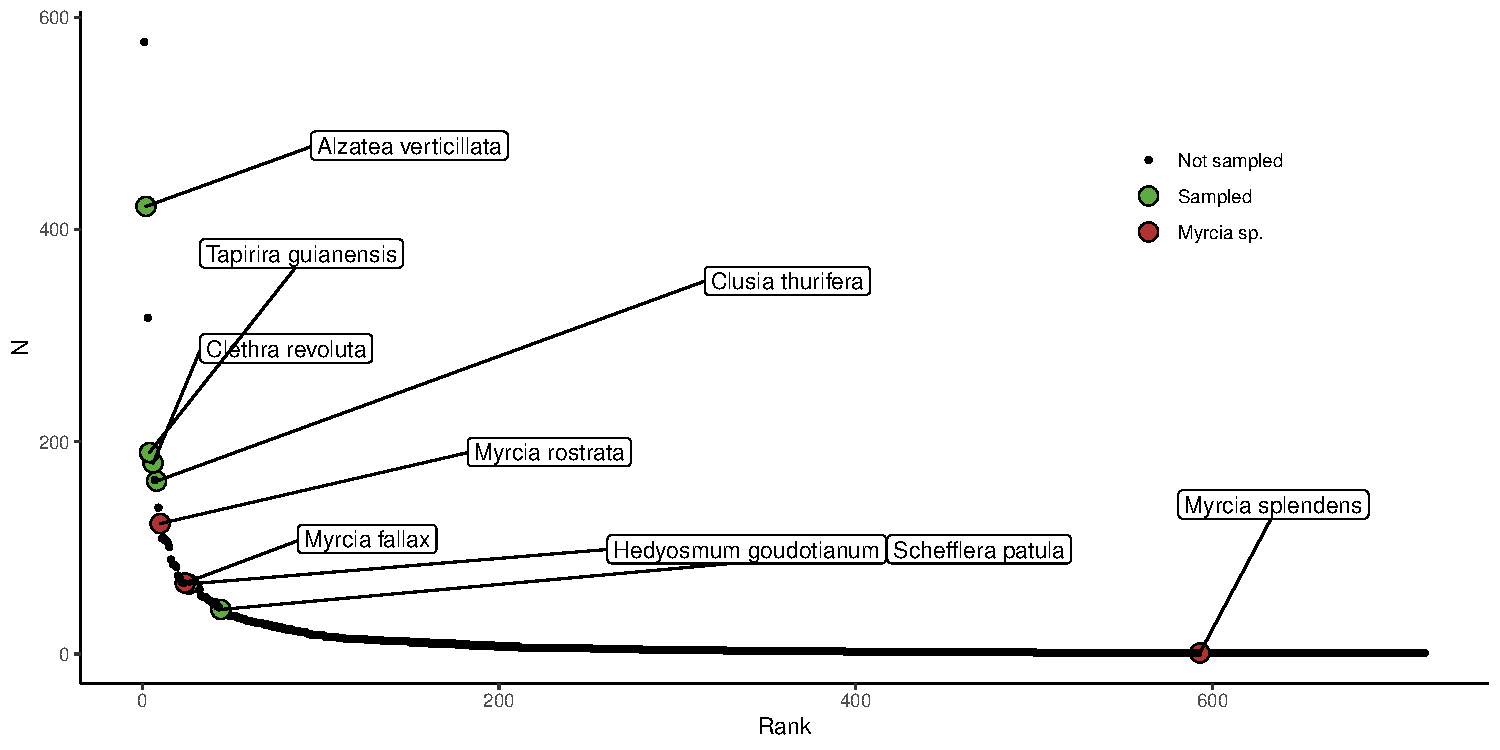
\includegraphics[width=\textwidth]{rank_abund}
\centering
\caption{Rank abundance curve of all individuals \textgreater{}10 cm DBH of all species found in the plots measured in this study. Census data from 2014 (ABERG, unpublished data). Species sampled as part of this study are highlighted in red. \textit{Myrcia} species which form the composite \textit{Myrcia} spp. are highlighted in green.}
\label{fig:rank_abund}
\end{figure}

\subsection{Sampling and Measurement}
Species were sampled in three plots representing the top, middle and bottom elevational extents of their ranges (Figure \ref{fig:ranges_ggplot}). Within each plot, a maximum of 10 seedlings were sampled. To minimise the chance of pseudo-replication of sampled seedlings, seedlings closer than 10 m to another sampled seedling were excluded from the analysis, as it could not be guaranteed that the stems were not connected by a stolon or rhizome. It also ensured that competition measurements were truly independent. Within a cluster of seedlings within 5 m of each other, each seedling was assigned a number and a random number generator was used to choose a single seedling for measurement.

Proxies for photosynthetic efficiency were measured on the highest fully-expanded leaf of each seedling. Leaf photosynthetic efficiency can be used as an indicator of physiological stress levels. Plants with a lower photosynthetic efficiency are more stressed than those with a higher efficiency. Chlorophyll-$\alpha$ fluorescence was measured using a Walz Mini-PAM II (Walz Effeltrich, Germany), on a randomly selected area of adaxial leaf surface, avoiding prominent leaf veins according to \citep{}. Chlorophyll-$\alpha$ measurements were used to calculate $F_v/F_m$ according to \citet{Genty1989}:

\begin{equation} \label{eq:fvfm}
F_v/F_m = (F_m - F_o)/F_m
\end{equation}

Where $F_m$ is the maximal fluorescence in the dark and $F_o$ is the minimal fluorescence in the dark \citep{Maxwell2000}. Fluorescence measurements were taken after exposing the seedling to 30 minutes of total darkness, to ensure complete dark adaptation \citep{Campbell2007}. Dark-adapted $F_v/F_m$ measures the photosynthetic capacity of the leaf by relaxing the reaction centres prior to the fluorescence measurement. $F_v/F_m$ is preferable to other chlorophyll fluorescence measures as it removes the noise created by environmental conditions at the time of measurement, instead providing a measure of the underlying photosynthetic capacity. A reduction in $F_v/F_m$ is indicative of plant stress. Here, individuals with $F_v/F_m$ values \textless{}0.7 are considered to be experiencing stress \citep{Maxwell2000}. 

In addition to $F_v/F_m$, leaf chlorophyll content was measured using a multi-spectral SPAD-meter (Minolta SPAD-502Plus, Spectrum Technologies, Plainfield, Illinois, USA). To account for variation in chlorophyll content across the leaf \citep{}, SPAD measurements were taken at three random points on the leaf. The leaf midvein, other prominent veins, and areas of obvious leaf necrosis were avoided in these measurements. The mean of the SPAD values was used to calculate an estimate leaf chlorophyll content using the conversion factor outlined in \citet{} for tropical broadleaf tree species:

\begin{equation} \label{eq:chl-spad}
Chl_\alpha = 0.53e^{\begin{matrix} 0.0364 \times \overline{SPAD} \end{matrix}}
\end{equation}


\subsection{Leaf and whole-plant morphological measurements}

\subsection{Competition measurements}

To assess adult-seedling competition interactions we used two metrics, Leaf Area Index of canopy foliage, and a metric approximating the degree of crowding from surrounding adult trees. Leaf Area Index (LAI) was calculated from hemispherical photographs of the forest canopy above each seedling. Photographs were captured under uniformly overcast cloud conditions to avoid lens flare and to aid in delineation of foliage from sky during processing \citep{Frazer2001}. Images were taken with a Coolpix 4500 compact camera, with a Nikon FC-E8 hemispherical fisheye converter lens. Images were constrained to a 60\textdegree{} circular azimuthal field of view in order to restrict LAI calculations to the part of the sky where the majority of photosynthetically active radiation penetrates the canopy \citep{Jupp2009, Jonckheere2005}. Images were then converted to 8-bit grayscale and binarized manually in ImageJ Version 1.51 \citep{} to separate sky from plant material. Binarized images were then analyzed using Hemiphot \citep{} in R to estimate LAI as the projected leaf area per unit ground area (m\textsuperscript{2} m\textsuperscript{-2}).

To approximate crowding from adult trees, we used an adapted version of the Iterative Hegyi Index \citep{Hegyi1974, Lee2004, Seifert2014}. Our adapted `Iterative Seedling Index' ($ISI$) uses adult tree trunk diameter at \textapprox{}1.3 m from ground level (Diameter at Breast Height, DBH) and the distance of trees from the seedling to calculate an index for each seedling. Higher $ISI$ values may result from combinations of  greater adult tree DBH and adult trees being closer to the seedling, higher values indicate greater competition pressure from surrounding adult trees:

\begin{equation}
\label{eq:ISI}
ISI_i = log(\sum_{j=1}^n (\frac{1}{{DIST_i}_j} D_j))
\end{equation}

where $D_j$ is the DBH of a competitor tree and ${{DIST_i}_j}$ is the euclidean distance between seedling $i$ and competitor tree $j$. $ISI$ was log transformed for analysis, as results spanned multiple orders of magnitude. The `iterative' aspect refers to the selection of competitor trees. An iterative selection method for competitive trees assumes that if the path between two trees is blocked by some obstacle, \textit{e.g.} another tree, the intensity of competition between them will be greatly reduced \citep{Gadow1999}. The radius around the seedling is divided into 12 30\textdegree{} sectors, where only the nearest tree \textgreater{}10 cm DBH within each sector is measured (Figure \ref{fig:hegyi}). The size of the competition radius ($C_R$) is defined as:

\begin{equation}
\label{eq:CR}
C_R = 2 \times \sqrt{\frac{10000}{N}}
\end{equation}

where $N$ is the number of trees \textgreater10 cm DBH per ha (stand density). Stand density data was taken from ABERG census data within each plot (ABERG unpublished data) and used to interpolate the value of $C_R$ for plot VC, for which no stand density data exists. We fitted a linear regression between the elevation and trees ha\textsuperscript{-1} of each plot, and interpolated the trees ha\textsuperscript{-1} of plot VC using the regression fit (Figure \ref{comp_radius_fit}). $C_R$ was rounded to the nearest metre for ease of measurement (Table \ref{table:CR}). 

\begin{figure}[H]
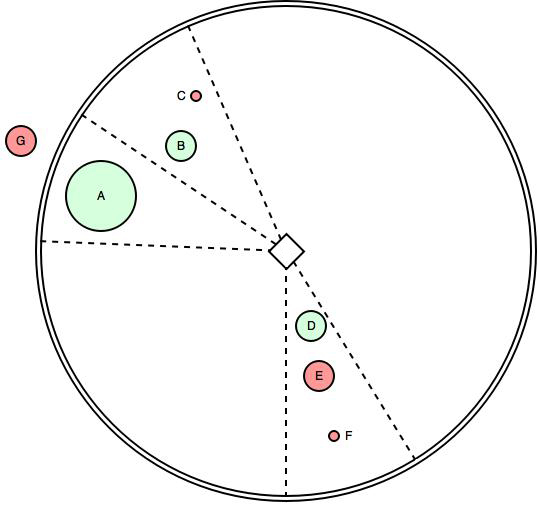
\includegraphics[width=0.5\textwidth]{hegyi}
\centering
\caption{Schematic diagram showing the iterative selection of active competitor trees for the Iterative Seedling Index (ISI) (Equation \ref{eq:ISI}). Trees marked in green (A, B, D) are active competitors for the tree of interest (black diamond). Trees marked in red (C, E, F, G) are non-active competitors, coloured circle radius represents tree DBH. The double circle defines the Competition Radius ($C_R$) (Table \ref{}, Equation \ref{eq:CR}). Dashed lines represent 30\textdegree{} zones within which to choose one active competitor. D is the active competitor of its zone as it is the nearest competitor of a suitable DBH (\textgreater{} 10 cm). F is not an active competitor as it is \textless{}10 cm DBH. G is not an active competitor as it is outside the competition radius. Adapted from \citet{Lee2004}.}
\label{hegyi}
\end{figure}

\begin{figure}[H]
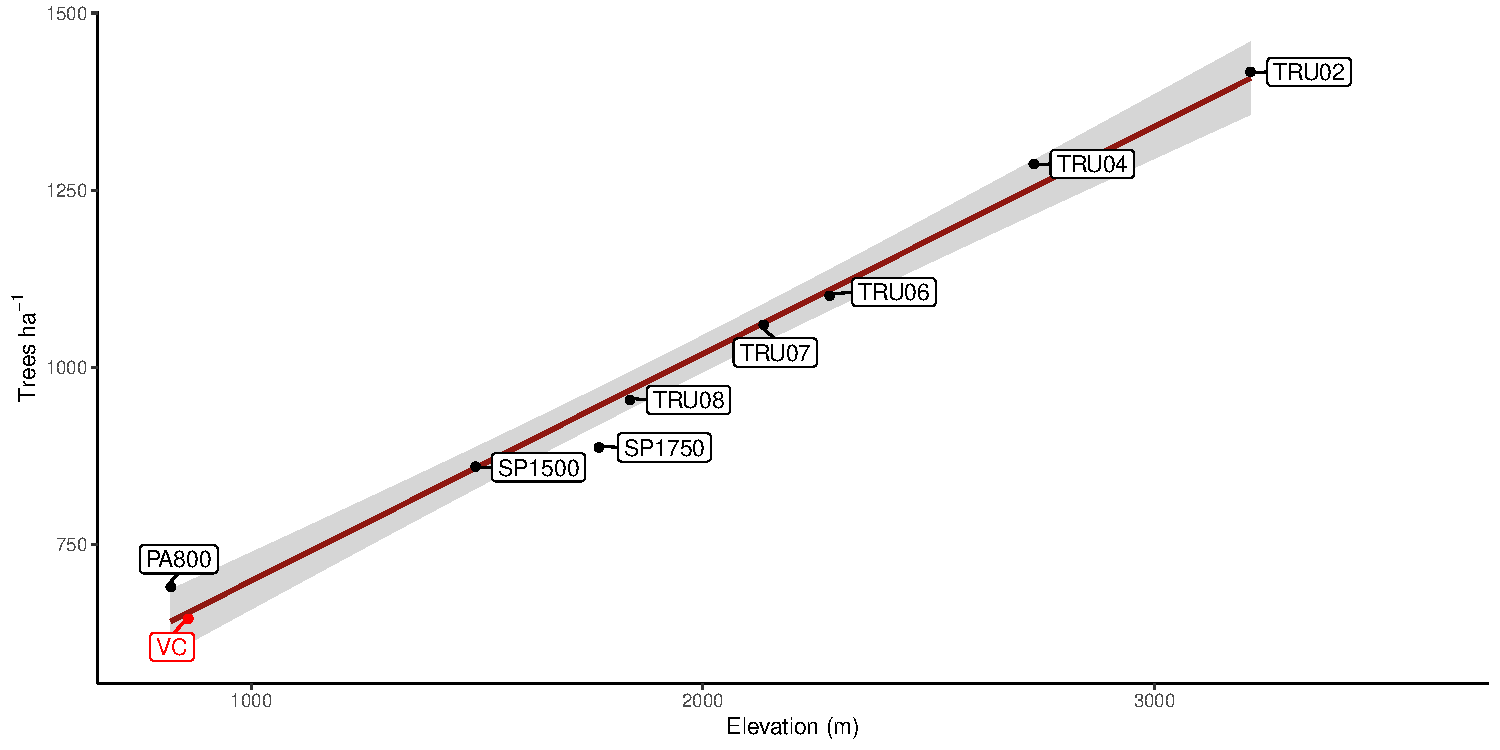
\includegraphics[width=\textwidth]{comp_radius_fit}
\centering
\caption{Linear regression with 95\% confidence interval of number of trees per hectare for each site, used to estimate number of trees per hectare for site VC. $R^2$ = 0.896, $F_{(1,7)}$ = 579.5, $p$ \textless{} 0.001.}
\label{fig:comp_radius_fit}
\end{figure}

\begin{figure}[H]
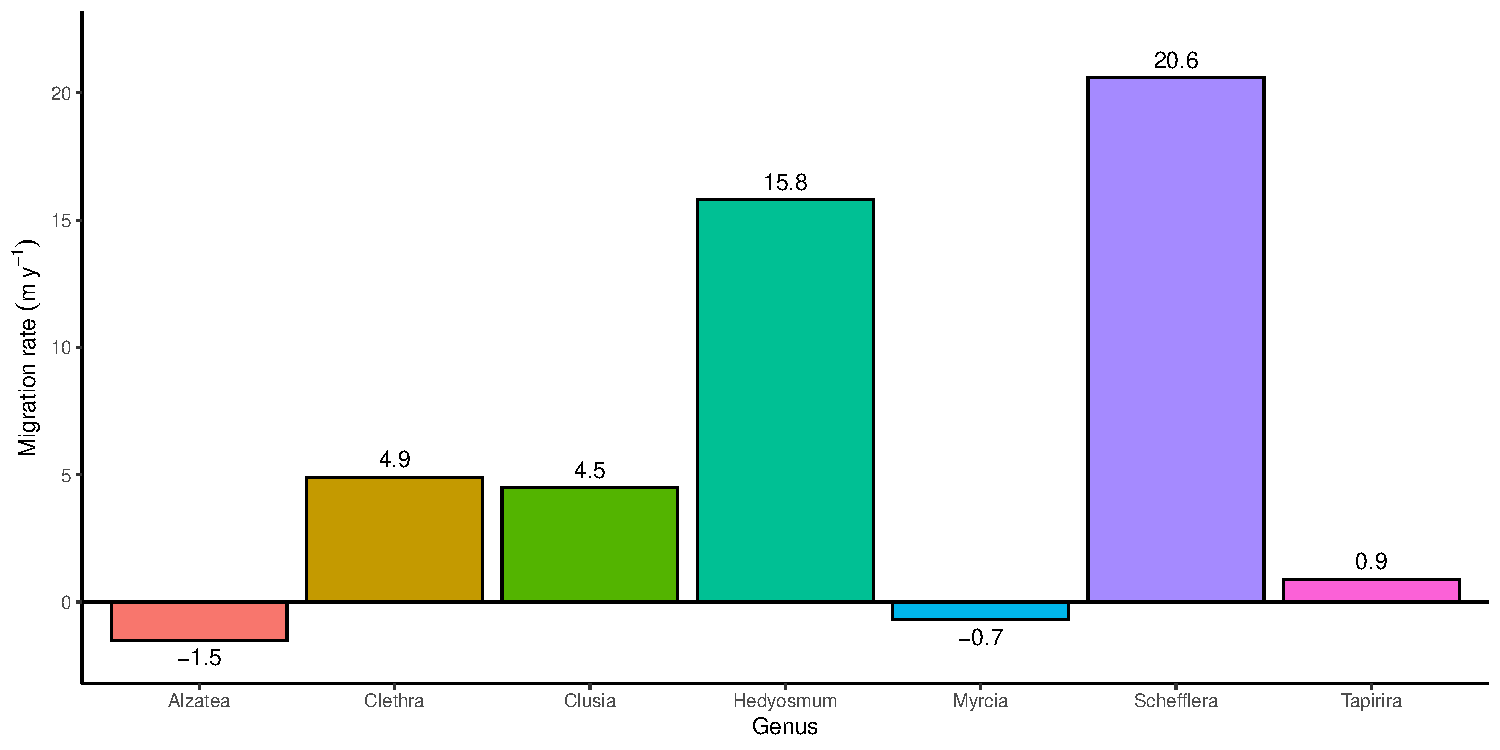
\includegraphics[width=\textwidth]{mig}
\centering
\caption{Estimated elevational migration rates within the Kos\~{n}ipata valley for selected genera of which species are studied here. Migration rates are estimated using shifts in the centre of gravity of tree basal area as measured in the ABERG 1 Ha plot network.}
\label{fig:comp_radius_fit}
\end{figure}

\subsection{Statistical Analysis}

A matrix of single predictor linear mixed effects models were compared to test for the presence and strength of the causal relationship between each of the two competition variables and each of the six plant traits. The fixed effect of elevation was also included in order to compare the effects of competition to that of elevation. All fixed effects were standardised to allow easy comparison of effect sizes, according to \citep{Gelman2008, Grueber2011, Gelman2018}. Model comparison was performed on models fitted using Maximum Likelihood (ML) estimates \citep{Bolker_weevils}. Model quality was compared using Akaike Information Criteria ($AIC$) \citep{Akaike1992}, Akaike weights ($W_i$), and fixed effect marginal pseudo-R\textsuperscript{2} values ($R_M^2$). 

In order to inform the error structure of single fixed effect mixed effects models, error structures of were compared using $AIC$ values on pairs of single fixed effect linear mixed effects models, where the slopes of each species were allowed to vary by either intercept or by slope and intercept, to show whether species differ appreciably in their trait response to the various competition variables and elevation (fixed effects) (Figure \ref{fig:traits_dAIC}, Appendix III). Where $\Delta{}AIC_{rsri}$ scores between pairs of models were -2\textless{}$\Delta{}AIC_{rsri}$\textgreater{}2 a random intercept structure was maintained in the single fixed effect models, in order to maximise parsimoniousness. Models reported in the results use the optimal error structure.

The best quality single fixed effect models (using either independent intercepts or slopes for each species) were compared using $\Delta$AIC\textsubscript{r} against a random effects model,  the variance explained by the whole model ($R_C^2$) and the fixed effects ($R_M^2$) using the \textit{MuMIn} package \citep{MuMIn_weevils}, and slope coefficients (Figure \ref{fig:daic_r2c_traits}, Figure \ref{fig:slope_traits}) to compare their relative effect on plant traits. 

\begin{equation}
\label{eq:model}
Y_{ij} = \beta_{0} + \beta_{1}X_{ij} + u_{0j} + u_{1j}X_{ij} + \epsilon_{ij}
\end{equation}

where $Y_{ij}$ is the response variable of species $i$ at site $j$, $X_{ij}$ is the fixed effect value of species $i$ in site $j$.

%model<-lmer(Y ~ 0+Dose:Substance+(0+Dose:Substance| Subjects), data= DoseResponse, na.action = na.exclude)


The random intercept grouping effect of site was used to account for pseudo-replication in site characteristics for seedlings sampled along the elevation gradient.

To better understand the potential multiplicative effects of competition variables we also compared linear mixed effects models with combinations of fixed effects, using $AIC$, $W_i$ and $R_M^2$, to find the model which best explained variation in each plant trait.

To understand variation between species in their physiological and morphological response to competition effects, slopes for each species were calculated and compared in the best fitting linear model, re-estimated using Reduced Maximum Likelihood (REML). 



All statistical analyses were conducted using R, version 3.2.4 \citep{R2019}. Linear mixed effects models were conducted using the \textit{lme4} package \citep{Bates2015}.

\section{Results}

\subsection{Variation in plant traits across elevation}




\begin{figure}[H]
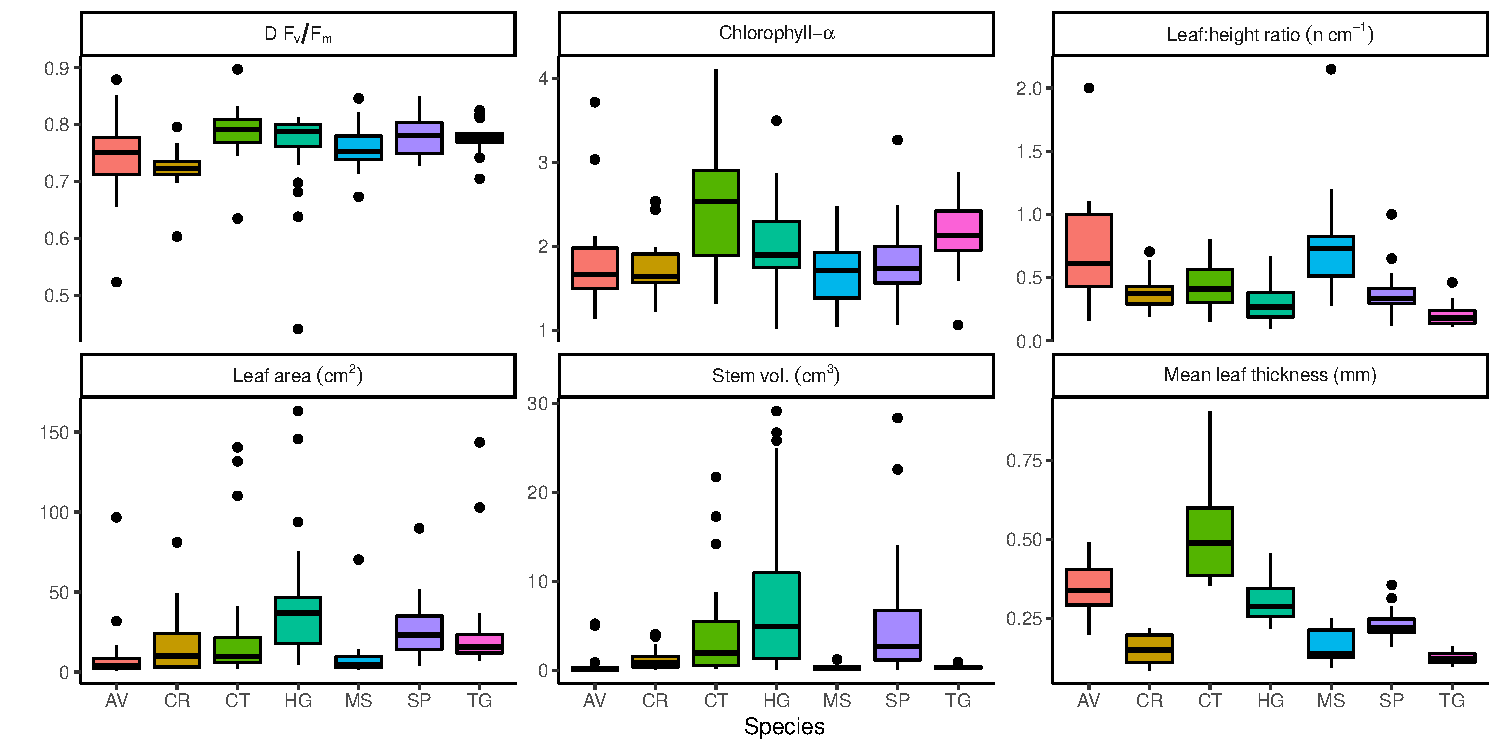
\includegraphics[width=\textwidth]{box}
\centering
\caption{Box plots showing the variation in plant trait values within each species.}
\label{fig:box}
\end{figure}

\begin{figure}[H]
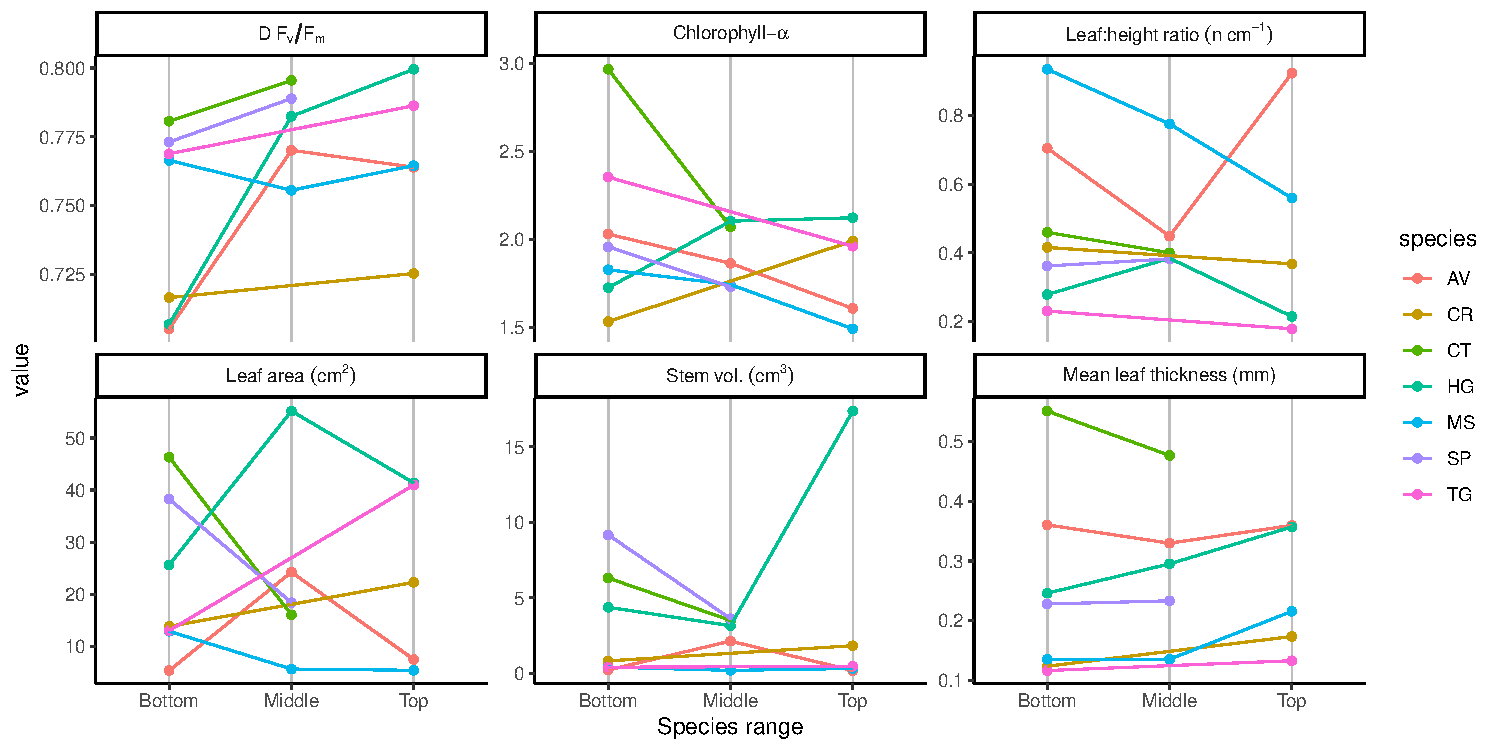
\includegraphics[width=\textwidth]{spaghetti}
\centering
\caption{Interaction plots showing the variation in plant trait values within each species.}
\label{fig:spaghetti}
\end{figure}


\begin{figure}[H]
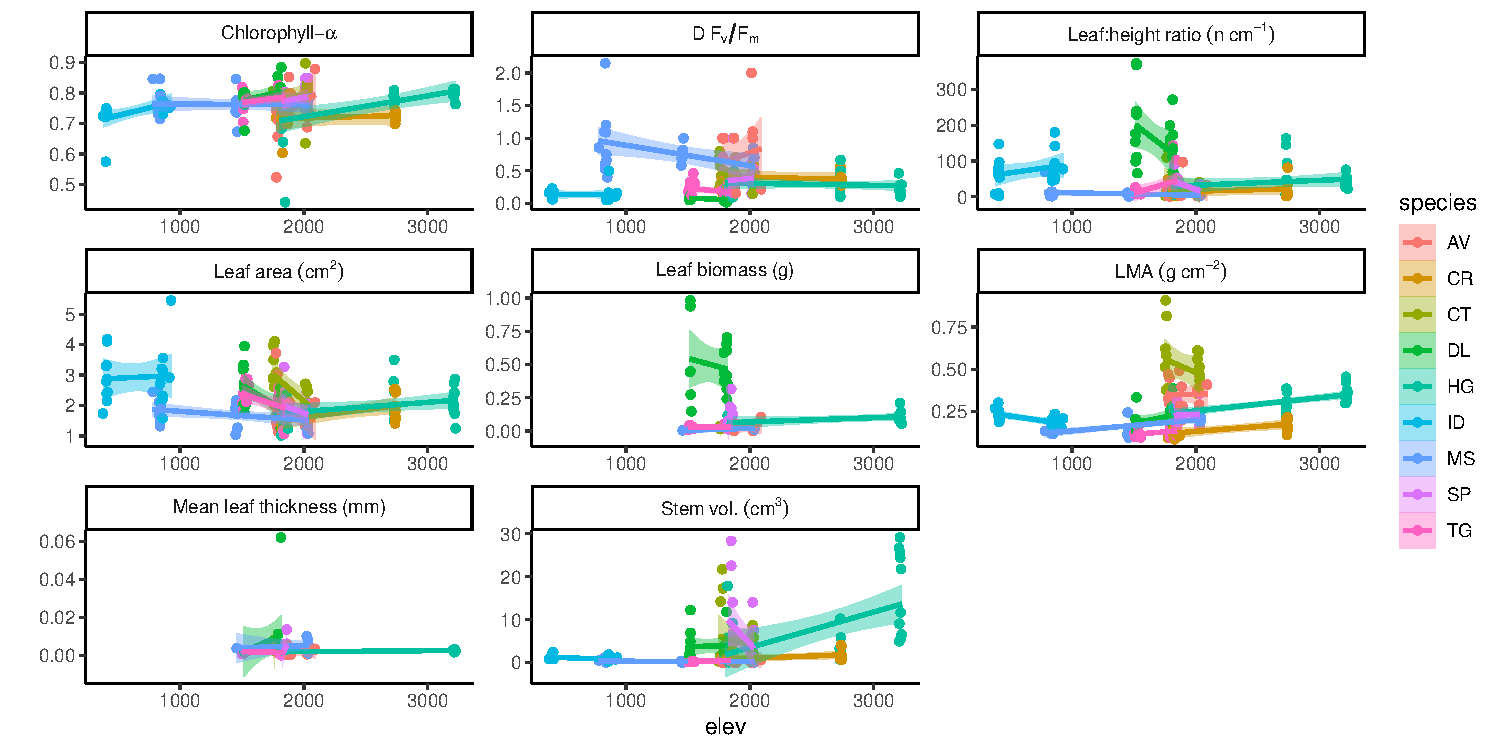
\includegraphics[width=\textwidth]{traits_elev_scatter}
\centering
\caption{Scatter plots with linear model fits for each species, showing the variation in plant stress variables and plant traits across elevation.}
\label{fig:traits_elev_scatter}
\end{figure}


\begin{figure}[H]
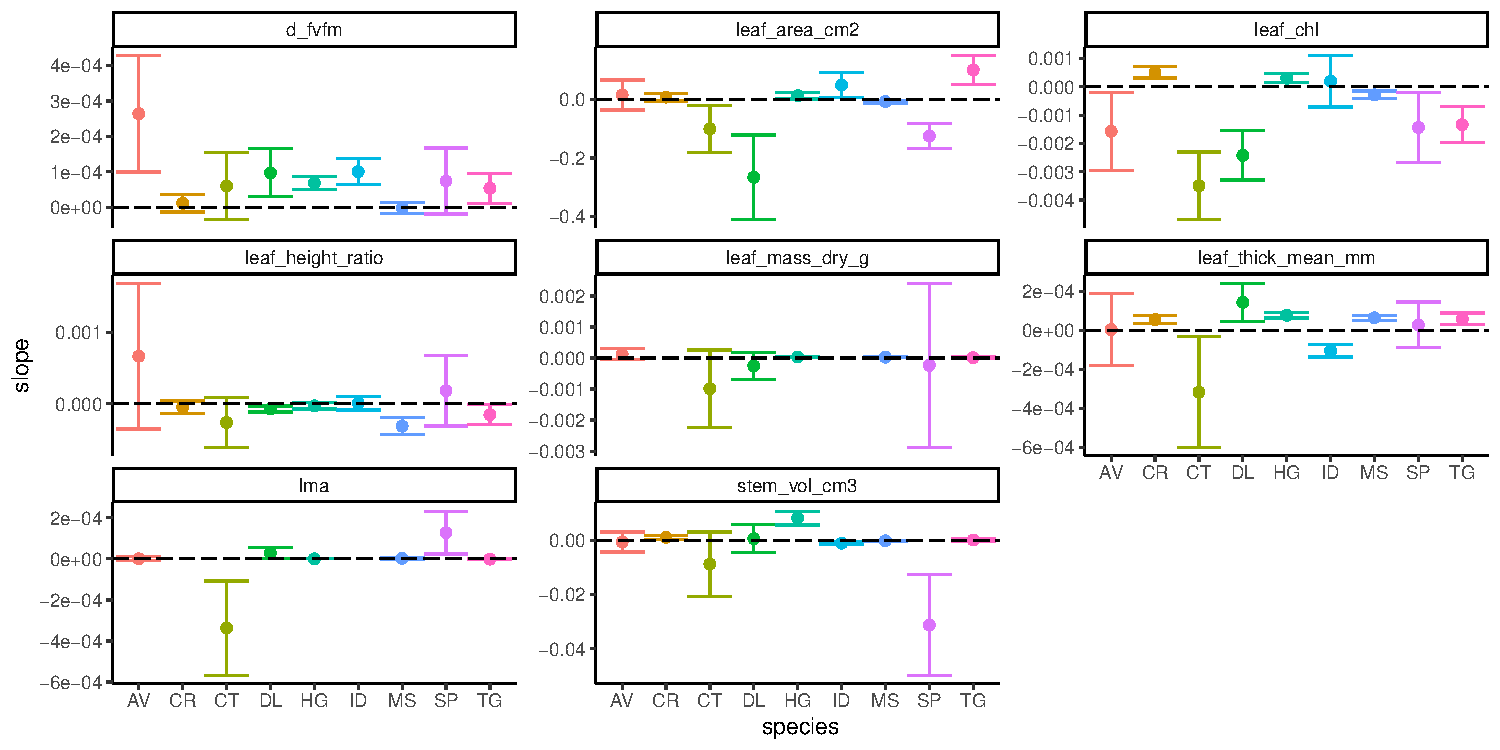
\includegraphics[width=\textwidth]{traits_elev_slopes}
\centering
\caption{Interval plots showing the effect sizes (slopes) of each fixed effect in single fixed effect linear mixed effects models of plant traits against forest structure variables and elevation, for comparison.}
\label{fig:traits_elev_slopes}
\end{figure}

\begin{figure}[H]
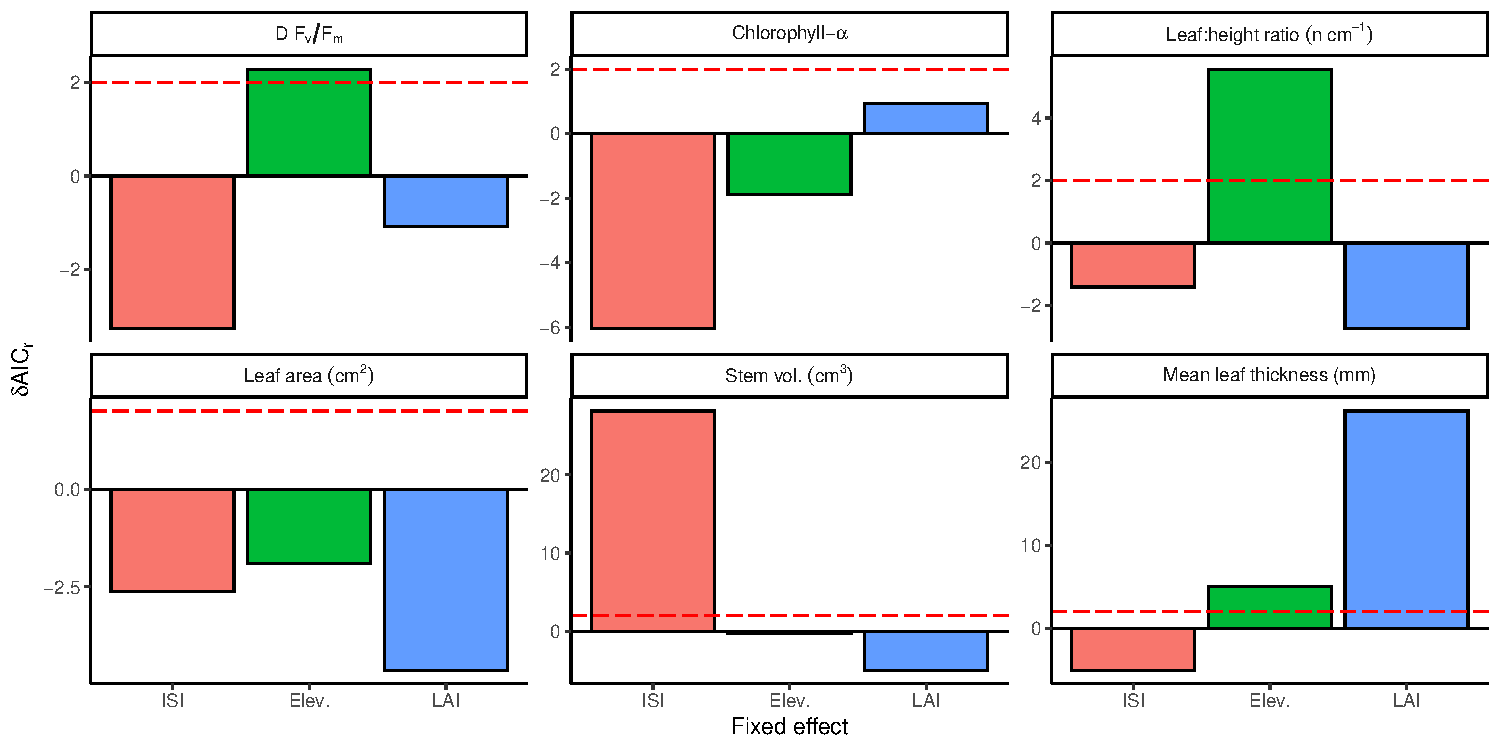
\includegraphics[width=\textwidth]{single_pred_daic}
\centering
\caption{The difference in AIC values between each single fixed effect model and a corresponding random effects model using no fixed effects. A higher $\Delta$AIC\textsubscript{r} means the model is of higher quality than the random effects model. Horizontal dashed red line indicates the level at which a model is not appreciably better quality than the corresponding random effects model.}
\label{fig:single_pred_daic}
\end{figure}

\begin{figure}[H]
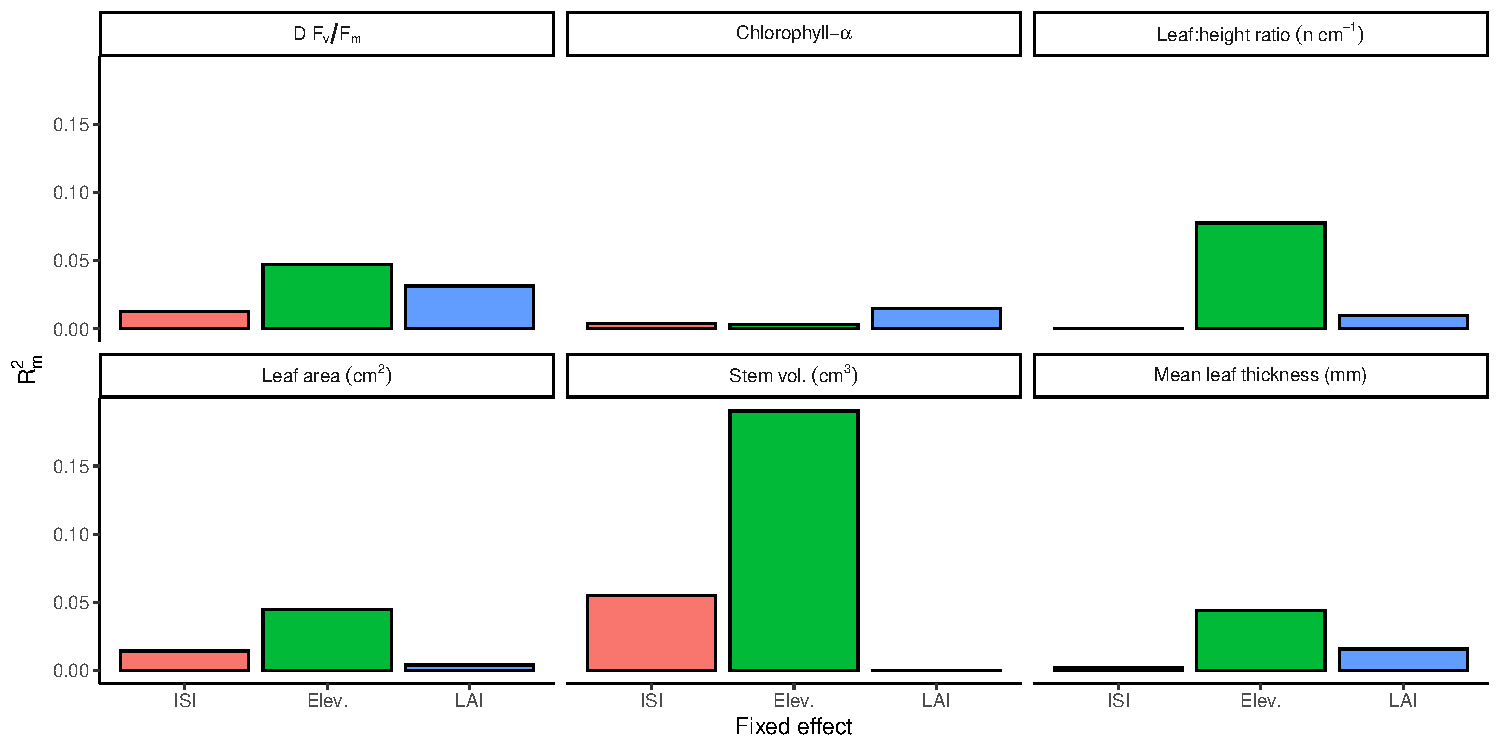
\includegraphics[width=\textwidth]{single_pred_r2m}
\centering
\caption{The variance explained by each single fixed effect model. The pale bars indicate the variance explained by the whole model while the bold bars indicate the variance explained just by the fixed effect in the model.}
\label{fig:single_pred_r2m}
\end{figure}

Table \ref{tab:best_fit_multi} shows the fixed effects and model fit measures from the best fitting multiple fixed effect models used to predict plant traits. For plant traits where one or more of the single fixed effect models was better when using a random slope (Figure \ref{fig:traits_dAIC}), the species slopes were allowed to vary for those fixed effects (Table \ref{tab:best_fit_multi}) in some model iterations. 

\begin{figure}[H]
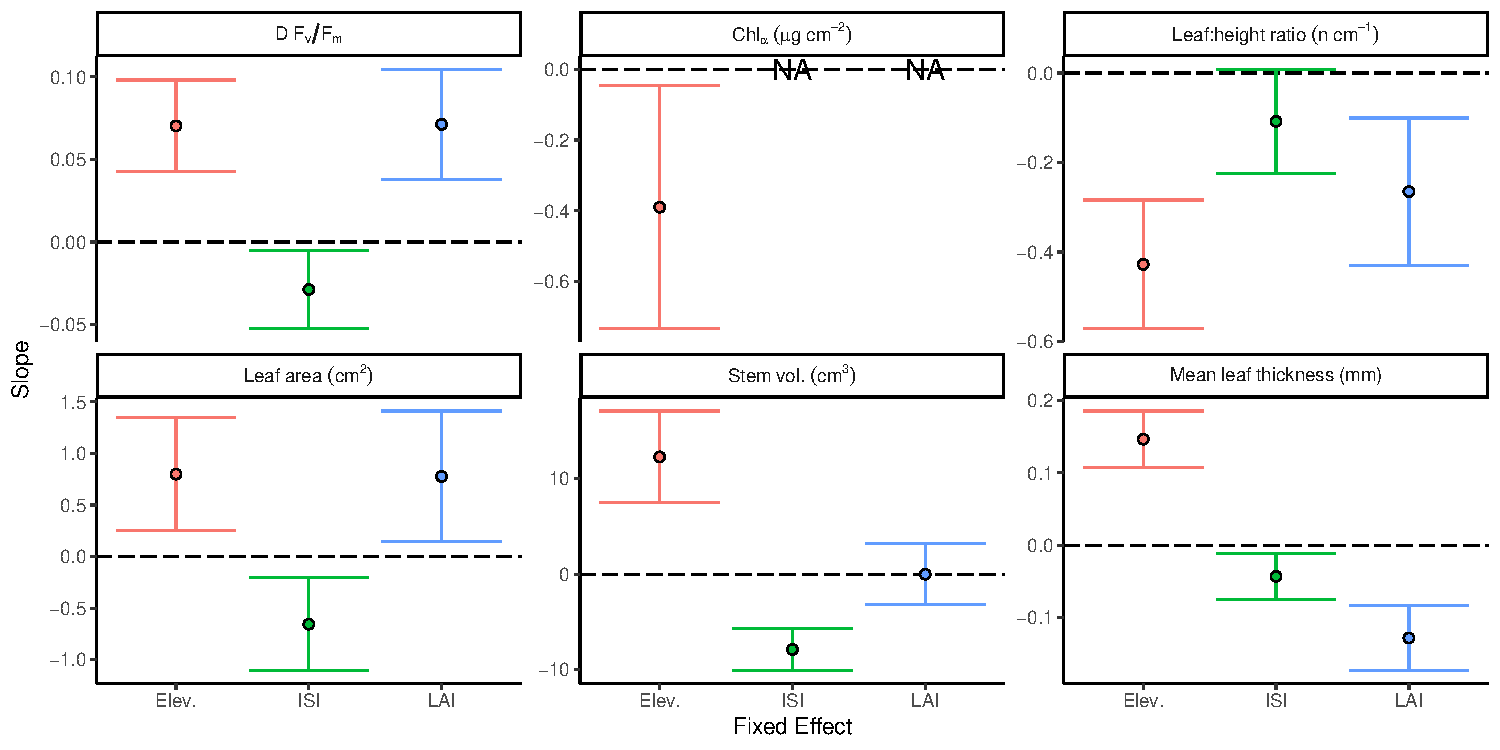
\includegraphics[width=\textwidth]{multi_pred_slope}
\centering
\caption{}
\label{fig:multi_pred_slope}
\end{figure}

All of the best models except the one predicting SPAD included elevation as a fixed effect alongside competition variables. All of the best models were better than a model using only elevation (Appendix IV). The best models for leaf:height ratio, leaf area and stem volume used random slopes for all the fixed effects identified as varying among species in the single predictor models. The fixed effects in the multiple fixed effect models still accounted for a small percentage of the variation in plant traits, ranging from 0.4\% (SPAD), to 17.3\% (stem volume).

When multiple fixed effects were used in a model, the standard errors surrounding the slopes of those fixed effects were reduced (Figure \ref{fig:fix_eff}, Appendix II). The effect of herbaceous plant abundance became larger in the multiple fixed effects model compared to the single fixed effect model. The best LMM for SPAD was no better than a random effects model ($\Delta$AIC\textsubscript{r} = -1.0) and was 14.2\% likely to be better than the next best model, which included only elevation ($W_i$ = 0.142).

\subsection{Effects of competition on plant traits}

Linear mixed effect models of the relationship between adult tree competition variables and plant traits outperformed equivalent random effect models in \todo{15/24 cases}, \textit{i.e.} those with a $\Delta$AIC\textsubscript{r}>2. However, the competition variables only accounted for a small percentage of the variance in each plant trait. The the highest $R_M^2$ in these single fixed effects models was the effect of Iterative Seedling Index on stem volume ($R_M^2$ = 4.3\%), despite the model as a whole explaining 56\% of the variation in stem volume. A similar effect is seen in all the other single fixed effect models, suggesting that unmeasured site specific effects are responsible for a large portion of the variation in plant traits.

The best fitting multiple fixed effect models all included the effects of elevation, Iterative Seedling Index and Leaf Area Index to explain variation in plant traits, except leaf chlorophyll content, which only included Leaf Area Index. 


\section*{Discussion}

This study aimed to (a) determine whether plant traits were affected by competition variables, (b) assess how the effects of competition compared to that of elevation, and (c) assess the degree to which plant trait-elevation relationships vary among species. It was found that competition variables never influence a given plant trait more than elevation. Adult-seedling competition effects (LAI and ISI) affect plant traits more than seedling-seedling competition (herbaceous plant abundance). LAI and ISI have contrasting effects on plant traits.

\section{Effect of competition and elevation on plant traits}
Single fixed effect models demonstrated that the three competition variables influence some plant traits ($\Delta$AIC\textsubscript{r} >2, Figure \ref{fig:daic_r2c_traits}a). The effect size of individual competition variables however, did not exceed that of elevation for any plant traits (Figure \ref{fig:daic_r2c_traits}b, Figure \ref{fig:slope_traits}).  The three competition variables, which represent different types of competition, vary in their effects on seedling traits.
\subsection*{Leaf physiology}
Together, SPAD and $F_v/F_m$ are useful measures of a plant's health and the integrity of its photosynthetic apparatus \citep{Clark2000}. SPAD is used as a proxy for leaf chlorophyll content \citep{Richardson2002}, while $F_v/F_m$ measures the efficiency with which a leaf can utilise light for photosynthesis \citep{Maxwell2000}. This study found contrasting effects of elevation on SPAD and $F_v/F_m$. As elevation increased, photosynthetic efficiency increased but chlorophyll content decreased slightly (Figure \ref{fig:slope_traits}). There is however, large variation in SPAD within sites and elevation explains little of the variance in SPAD (Figure \ref{fig:trait_elev}), meaning this relationship may be erroneous. Competition variables explained comparatively little variation in $F_v/F_m$ or SPAD compared to morphological leaf traits (Figure \ref{fig:trait_elev}b).

\subsubsection*{Photosynthetic efficiency}
Single fixed effect models showed that an increase in canopy density (LAI) caused an increase in photosynthetic efficiency ($F_v/F_m$) (Figure \ref{fig:slope_traits}). Specifically, an increase in photosynthetic efficiency under denser canopy may be the result of a more temporally constant microclimate \citep{Amissah2015}. A denser canopy regulates diurnal temperature oscillations by more effectively trapping warm air between the canopy and the forest floor, reducing temperature stress on the plant \citep{Larcher2003}. Increased shading under denser canopy also reduces the potential for seedling desiccation and cavitation, which can cause damage to seedling leaves. As Sun-flecks move across the forest floor they result in rapid leaf temperature increase \citep{Rozendaal2006, Poorter2010}. Additionally, a reduction in direct sunlight reduces the potential for UV-B damage to photosynthetic apparatus \citep{Dobrikova2013}. Diurnal temperature oscillations are generally of greater range at higher elevations \citep{Seidel2005} as is the UV-B insolation fraction \citep{Piazena1996}, suggesting that the beneficial effects of increased canopy density on photosynthetic efficiency may become greater at higher elevations. In this region however, persistent cloud cover at higher elevations throughout the day may result in no increase in incident UV-B, the majority being absorbed by cloud condensation nuclei before it reaches the leaf \citep{Flint2003}.

Canopy density decreases with elevation (Figure \ref{fig:env_elev}), though this trend may be the result of wide within site variance ($\Delta$AIC\textsubscript{r} < 2). This trend concurs with more conclusive results from other studies which show a clear decrease in canopy density with elevation \citep{Kitayama2002, Moser2008}. The more variable relationship seen in this study may be the result of bias in the sampling strategy. LAI was not measured systematically across each site, instead being measured above each sampled seedling. It is expected that seedlings will grow successfully only under canopy where the average light intensity falls between a minimum needed for growth and a maximum that ensures temperature and UV-B stress does not cause the seedling to perish. In this study therefore, extreme canopy densities were probably not sampled. The presence of bias in our sampling strategy is supported by comparing the range of LAI measurements in other studies. For example, \citet{Asner2003}, in a review of 61 tropical evergreen forests, found that LAI ranged from 1.5 to 8. (after outlier exclusion), whereas our LAI estimate ranged from only 1.0 to 5.5, implying that a representative LAI sample was not achieved within each plot.

It is expected that a decrease in canopy density with elevation will lead to more individuals showing signs of stress at higher elevations, due to the factors discussed above. An increase in plant stress limits overall fitness as energy is allocated more to acclimation processes than to fecundity \citep{Reu2011}. This may hinder further upward migration, especially in species with limited dispersal distance such as \textit{I. deltoidea} which relies on seed dispersal by large mammals (predominantly primates) \citep{Russo2005, Kuprewicz2013} over short distances. In this instance however, there is no clear decrease in $F_v/F_m$ with elevation within any species ($\Delta$AIC\textsubscript{r} = 1.61), with 8/9 species show an increase in $F_v/F_m$ with elevation (Figure \ref{fig:trait_elev}). This suggests that the effect of canopy density in decreasing photosynthetic efficiency across elevation is masked by other environmental variables.

%It must be noted that while there is a positive relationship between photosynthetic efficiency and LAI in this experiment, this does not necessarily equate to an overall increase in photosynthetic rate. As LAI increases, PAR decreases, meaning that at some point, the beneficial effects of canopy cover will be masked by the detrimental effects of shading, leading to a net reduction in biomass accumulation for the seedling and a concurrent decrease in fitness (REF).

In contrast to the effects of LAI, ISI caused a decrease in photosynthetic efficiency. This suggests that the mechanisms by which LAI may affect photosynthetic efficiency (shading, temperature regulation) differ from those of ISI (nutrient competition, water competition, predation mutualisms) \citep{Lewis2000}. Other studies have shown a nutrient competition effect between adult trees and nearby seedlings. \citet{Palik1997} demonstrated that adult trees of greater basal area (equivalent to DBH) cause a larger reduction in soil available nitrogen which subsequently decreased the growth of pine seedlings. Similarly, \citet{Barberis2005} showed that trenching around neotropical tree seedlings in order to decrease root competition increased the growth and leaf nutrient content of the seedlings. In this set of plots, soil moisture is rarely a limiting factor, and insect predators are much rarer in cloud forests than lowland forests \citep{Rodriguez-Castaeda2010}. This suggests that any negative effect of increased ISI on photosynthetic efficiency would be the result of nutrient competition by adult trees.

ISI decreases with elevation (Figure \ref{fig:env_elev}) and a decrease in ISI causes an increase in photosynthetic efficiency. The increase in $F_v/F_m$ with elevation may therefore be partly the result of decreased adult-seedling nutrient competition at higher elevations. The large effect of elevation however, implies that other unmeasured environmental variables influence this trend more than simply  a decrease in ISI.

Herbaceous plant density had little effect on $F_v/F_m$. In the single predictor models, the slope was the smallest of all the environmental variables and explained the least variance (Figure \ref{fig:daic_r2c_traits}, Figure \ref{fig:slope_traits}). In the multi-predictor models the best fitting model did not include herbaceous plant density (Table \ref{tab:best_fit_multi}). Other studies have shown that size-asymmetric competition with adults has a much greater role in structuring forest ecosystems than seedling-seedling competition, especially in tropical forests where seedlings are relatively scarce compared to adult trees \citep{Moles2004, Powers2004}. \citet{Paine2008} estimated the area around tree seedlings in neotropical forests within which seedlings affect the availability of resources both above- and below-ground to other seedlings, finding that most zones did not overlap at all. This implies that seedling-seedling competition in neotropical forests is insignificant. 

\citet{Maxwell2000} suggest that generally, optimum $F_v/F_m$ is \textapprox0.83, and that if $F_v/F_m$ falls below \textapprox0.8, it is indicative of some kind of plant stress. It is important to note however, that this optimum is likely to vary markedly among species and has been criticised as yet another arbitrary threshold for a dynamic phenomenon \citep{Ghouil2003}. As a conservative estimate, here plants are defined as experiencing physiological stress when $F_v/F_m$ \textless{} 0.7. Figure \ref{fig:trait_elev} shows that only a few individuals fall below this threshold, suggesting that few individuals along the elevational gradient are experiencing stress. Only \textit{C. revoluta} features reduced photosynthetic capacity with elevation. \textit{C. revoluta} also has the most individuals below the 0.7 threshold. This could be evidence that \textit{C. revoluta} individuals experience greater stress at increasing elevations, but the relationship shown here is not strong enough to be conclusive, with large variation within each plot that \textit{C. revoluta} seedlings were sampled. Alternatively other species which feature an increase in photosynthetic efficiency may be experiencing stress at lower elevations, giving support for the hypothesis given by \citet{Campbell2007}, in which species ranges contract from the bottom up. Temperature increase is the most likely source of this increased stress at the lower limits of species ranges, though stress induced by antagonistic interactions from previously lower elevation species that have shifted upslope faster is also possible. Herbivores for example are expected to move upslope faster than tree species due to their mobility and shorter life-cycles \citep{Chen2011}.

\subsubsection*{SPAD}
SPAD value was not clearly influenced by any of the measured competition variables, or elevation (Figure \ref{fig:slope_traits}). SPAD varied largely both within and among species, with large standard errors surrounding the estimates of each species (Figure \ref{fig:trait_elev}, Table \ref{tab:plant_traits}). The best fitting multiple fixed effect LMM for SPAD did not include elevation (Figure \ref{tab:best_fit_multi}), though this model was only 14.2\% more likely to be the best model than the next best model and the fixed effect of LAI accounted for only 0.4\% of the variance in SPAD (Figure \ref{tab:best_fit_multi}). 

The lack of meaningful variation in SPAD contrasts other studies that have shown increases in chlorophyll content in response to shading \citep{Brand1997, Rijkers2000, Rozendaal2006, Dai2009, Zervoudakis2012} and soil nitrogen content \citep{Cechin2004}. In this study however, SPAD did not vary with LAI (shading), ISI (soil nutrient availability) or herbaceous plant abundance. 

The species with the smallest ranges show the steepest decrease in SPAD with elevation (Figure \ref{fig:trait_elev}). From this one could suggest that specialists are more sensitive to increases in elevation in terms of their photosynthetic apparatus. Species with small ranges are interpreted as being more specialist in their environmental requirements \citep{Thuiller2005}.

\subsubsection*{Summary}
Most species demonstrated an increase in $F_v/F_m$ with elevation, while SPAD showed little meaningful variation in response to elevation. Adult-seedling competition variables had contrasting effects on $F_v/F_m$ while seedling-seedling competition had no effect. A decrease in ISI with elevation may have contributed to the observed increase in $F_v/F_m$ with elevation though it is possible that this trend is actually a result of increased stress at lower elevations in response to temperature stress or herbivory stress. H\textsubscript{n1} is therefore accepted for SPAD and rejected for $F_v/F_m$. The best multiple fixed effect model for $F_v/F_m$ included all competition variables, H\textsubscript{n2} is therefore rejected for $F_v/F_m$. SPAD is predicted equally poorly by elevation and competition variables.
%---------------------------------------------------------------------------------------------------------------------------------------------------%---------------------------------------------------------------------------------------------------------------------------------------------------
\subsection*{Leaf and plant morphology}
Leaf thickness increased with elevation. Other studies have also found positive correlations between leaf thickness and elevation, identifying climatic drivers such as mean daily insolation and diurnal temperature variation \citep{Niinemets2001}, which lead to reduced leaf pay-back times and a need to grow leaves that can survive the more variable environmental conditions found at higher elevations \citep{Milla2011}. Increased UV-B results in an increase in cuticle thickness, to reduce the concentration of UV-B absorbed by photosystem II  (PSII) where it can cause damage and thus photoinhibition \citep{Vass1997, Szilard2007}. In this study however, it is unclear whether the insolation UV-B fraction does increase with elevation as it was not measured. Additionally, it is expected that frequent cloud immersion in the high elevation sites would reduce UV-B absorption and thus the need for thick cuticles. Leaf thickness decreased under increased canopy density (Figure \ref{fig:slope_traits}), adding support to the conclusion that increased direct sunlight is the cause of the decrease in leaf thickness with elevation.

Leaf area variation was explained poorly by both competition variables. Previous studies have shown a clear decrease in leaf area with elevation, citing decreases in canopy density and an increase in nutrient competition with elevation as drivers of this variation \citep{Pan2013}. Plants with access to higher resource levels generally invest in leaves which can achieve a higher photosynthetic rate per energy input in leaf construction, at the expense of leaf longevity \citep{Mediavilla2009}. In the plots studied here however, available nitrogen does not decrease with elevation, though elevational variation in other nutrients is not known.

Leaf:height ratio decreased with elevation (Figure \ref{fig:slope_traits}) meaning that plants became less leafy per unit stem height as elevation increased.  However this relationship explained very little of the variance in leaf:height ratio (Table \ref{tab:plant_traits}). Competition variables had little effect on leaf:height ratio (Figure \ref{fig:slope_traits}). Few studies have focussed specifically on measures of leaf:height ratio or number of leaves as an adaptive/acclimatory trait though we may interpret that a reduction in ``leafiness" is an extension of the trend seen in reduced leaf area with elevation. Seedlings may be more likely to produce fewer leaves in order to allocate more biomass to structural support in those leaves that are grown \citep{Onoda2011}.

Stem volume decreased with ISI (Figure \ref{fig:slope_traits}). This may have contributed to the increase in stem volume with elevation, as ISI decreases with elevation (Figure \ref{fig:env_elev}). Other studies have found that stem volume increases with average wind speed in order to provide greater stem support \citep{Onoda2011}, and that stems become more elongated as diurnal temperature range increases \citep{Myster1995}. Wind speed is expected to increase with elevation as is diurnal temperature range, providing further support for the trend seen here. An increase in stem volume with elevation suggests that tree seedlings are allocating less biomass to other parts such as the leaves, meaning that plant growth may be slower at higher elevations. This is supported by the negative relationship between leaf area and elevation, and the negative relationship between leaf:height ratio and elevation, which suggests that seedlings produce fewer, smaller leaves as elevation increases.

\subsection*{Summary}
Stem volume was the only morphological plant trait that showed clear variation with a competition variable (ISI), therefore H\textsubscript{n1} is accepted for all other morphological plant traits. All morphological plant traits were best explained by a multiple fixed effect model including elevation and a combination of competition variables, therefore H\textsubscript{n2} is accepted for all morphological plant traits. Morphological plant traits varied across elevation in a manner similar to that identified by previous studies, responding to elevation dependent abiotic environmental variables such as temperature and nutrient availability. The strength of the relationships seen here is not as great as that demonstrated by other studies, possibly because of the comparatively low sample size per species in this study compared to larger reviews and the presence of confounding environmental variables that were not accounted for in statistical analysis.

\section{Variation in plant traits with elevation}
Within each species, plant traits vary across elevation, with slope standard errors overlapping zero in only a few instances (Figure \ref{fig:trait_elev}). H\textsubscript{n4} can therefore be rejected, and it can be concluded that the individuals sampled in this study are acclimating their morphology in response to elevationally dependent environmental variables. The difference in magnitude and direction of the relationships shows that species are responding differently to changes in elevation. Supporting the observations and predictions of other studies that species are likely to migrate at different rates to climate change. Those species showing increased morphological change with elevation are expected to be more sensitive to changes in climate and are thus more likely to show greater migration rates.

\subsection*{Variation among species}
Species varied largely in the direction, magnitude and variance of their plant trait response to elevation (Figure \ref{fig:trait_elev}), therefore H\textsubscript{n5} is rejected. Variation among species in slope implies that species differ in their sensitivity to changing environmental conditions across elevation. \textit{D. lamarckianum} and \textit{I. deltoidea}, the two monocot species, show no similarity in their plant trait response to elevation, often having different slope directions for a given plant trait. Together, \textit{D. lamarckianum} and \textit{I. deltoidea} show no difference to dicot species in terms of their plant trait-elevation relationship. \textit{A. verticillata} has a comparatively large variance for all trait-elevation relationships except stem volume. This implies that \textit{A. verticillata} is either more sensitive to changes in climate, or that it has a larger acclimatory range than other species; both may be true. \textit{A. verticillata} has a very small elevational range (Figure \ref{fig:range_plot}) but is also one of the most common tree species found along this set of plots (Appendix VI). This supports the theory that common species have a wider acclimatory range and that species with small ranges are sensitive to environmental variation. In contrast, \textit{Myrcia} spp. has little variation in plant traits compared to other species but has the largest elevational range, the \textit{Myrcia} spp. species sampled are among the rarer species sampled.

Leaf thickness had a similar positive relationship with elevation in 7/9 species, whereas \textit{I. deltoidea} and \textit{S. patula} featuring reduced leaf thicknesses with elevation (Figure \ref{fig:trait_elev}). \textit{C. thurifera} had exceptionally high variance compared to other species, this is due to dense and prominent leaf vein structure in this species (Appendix V). For many \textit{C. thurifera} individuals, the diameter of the micrometer used to measure leaf thickness was too wide to be placed between the prominent leaf veins, leading to an over-estimation of leaf thickness for these individuals. Regardless, \textit{C. thurifera} showed a similar increase in leaf thickness with elevation. \textit{I. deltoidea} had the steepest decrease in leaf thickness over elevation (Figure \ref{fig:trait_elev}). This trend may be a peculiarity of the species or a result of environmental conditions at the upper sample plot for this species (VC). It is impossible to confirm whether site level variation at VC had a peculiar effect on \textit{I. deltoidea} leaf thickness as \textit{I. deltoidea} was the only species sampled at this site. Potentially, the greater leaf thickness at PA400 compared to VC is due to an adaptation to increased herbivory pressure at PA400. There is no evidence for this increase in herbivory in lowland plots other than a general trend that herbivory pressure decreases with elevation in tropical forests \citep{Rodriguez-Castaeda2010}.


\subsection*{Summary}
Tree seedlings are responding to changes in elevationally dependent environmental variables by altering their morphology. Additionally, the strength of the plant trait response varies between species, suggesting that some species are more sensitive to environmental change than others. 

The lack of a clear relationship between plant traits and competition intensity, suggests that tree seedlings are not affected by the biotic environment at the extremes of their ranges more than they are by other environmental variation. Species will therefore continue to migrate upslope, largely unimpeded by changes in biotic environment. It is possible that species will encounter biotic environmental thresholds beyond which adaptation and acclimation are no longer able to prevent stress and increased mortality. In order to answer these questions experimental transplantation is recommended, in order to place individuals outside of their current range. Even then, experimental transplantations do not account for potentially rapid micro-evolution that may occur as species migrate into novel environments. Sufficiently rapid micro-evolution could result in species being able to migrate upslope almost indefinitely, as they adapt and become more able to acclimate to changing climates.

\section{Predictions for future species migration}
This study confirms that adult-seedling competition intensity decreases with elevation (H\textsubscript{n3}), and that this decrease causes some proportion of the effect of elevation on plant traits, though this proportion is likely to be small as LMMs show that elevation still has the greatest influence over plant traits, despite including competition variables alongside elevation in multiple fixed effect models. As such, species may continue to move upslope as temperature increases, without being negatively affected physiologically at the upper limits of their ranges by adapting their morphology to the changing environment. The results from this study however, cannot be used to determine what will happen if a species reaches its adaptational limits as its range shifts. Given that few species experienced physiological stress, it is suggested that none of the species sampled have reached this limit yet. The exception being \textit{C. revoluta}, which shows some evidence of increased physiological stress with elevation and relatively flat relationships between elevation and plant traits, though this trend cannot be confirmed without more study.

Most species featured a decrease in photosynthetic efficiency at the bottom of their elevational ranges. This implies that these species may experience progressively greater plant stress at the bottom of their ranges as temperature increases, and the bottom of their range will continue to shift upslope as a result. This study cannot infer whether the contraction of species' lower range limits will be faster or slower than the expansion of the upper range limit, though other studies have suggested that lower range limits will shift upslope faster than upper limits \citep{Campbell2007}, owing to climate change proceeding faster than micro-evolutionary processes to adapt to higher elevations. This will lead to an overall reduction in range size for many species.

\section{Limitations of this study}
This study sampled seedling physiology over a narrow time period. While $F_v/F_m$ and SPAD are unlikely to vary on a daily basis, they may do over the course of a season \citep{Porcar-Castell2008}. Seedlings are likely to alter their leaf physiology and morphology in response to a temporally heterogeneous environment throughout the course of their life. As canopy gaps open and close the light and precipitation regime will change. The measured physiological responses of individuals therefore may not be representative of its physiology over a lifetime. Furthermore, this study only measured seedlings, ignoring other life stages. This means the results of this study cannot be used to directly infer the effects of biotic interactions on plant traits across entire populations. It is likely however, that established adult trees will be less sensitive to competition from other adult trees and completely insensitive to competition from seedlings \citep{Paine2008}. 

Nine tree species were selected for this study. Although these species are common in the areas we sampled (Appendix VI), there are many other species which may react more or less to the biotic environment. There is evidence that rare species are more affected by environmental factors \citep{Lyons2005,Mouillot2013}. Rare species are more likely to occupy specialist niches, which are narrower on a local geographical scale than those of generalist species \citep{Boulangeat2012}. The evolutionary histories of specialists means they are less likely to be able to acclimate to novel environments. Compared to the common species studied here, rare species will not have such a large direct effect on globally significant ecosystem services such as carbon sequestration, albedo, and drainage. This does not mean that rare species do not have the potential to heavily influence ecosystem services indirectly. \citet{Lyons2001}, and \citet{Lyons2005} found that less common species play vital supporting roles in maintaining ecosystem functions such as enhancing invasion resistance and making limiting resources available to other species  . 

There is large potential for falsely inferring causation from the results of this study. Along elevational gradients many environmental factors both abiotic and biotic co
vary. For example, this study concluded that an increase in ISI caused a decrease in photosynthetic efficiency. However, it was found that ISI covaries with elevation, along with many other potential unmeasured environmental variables, therefore photosynthetic efficiency may have merely inversely correlated with ISI rather than ISI causing the variation in photosynthetic efficiency, despite well-documented supporting evidence.

This study is deliberately wide in its scope, using competition intensity proxies in order to infer the influences of many ecosystem processes such as nutrient competition, shading, etc.. By not explicitly testing the effects of these mechanistic processes, which are complex in their effects, we cannot determine the relative contribution of each process implicit in each competition proxy. It is recommended therefore that experiments under constant environmental conditions explicitly test the effect of variation in ecosystem processes which are implied to change as a result of variation in the competition proxies measured here, such as nutrient availability and shading.

The study did not use experimental treatments. It could be argued therefore that measured seedlings would have been unlikely to show stress at all, as seedlings would not have grown to the minimum size needed for measurement otherwise.

\section{Further research}
On the basis of this study, which shows that adult-seedling competition intensity varies across elevation and that this variation forms part of the observed plant trait response to elevation, it is recommended that future studies aim to identify competition intensity thresholds beyond which individuals cannot acclimate to the environmental conditions. The location of thresholds should be confirmed using experimental transplantation of seedlings to different elevations to observe variation in plant traits.

In order to determine whether changes in competition intensity also affect adult trees, and thus recruitment, similar studies should be performed on adult trees. This would help to improve the accuracy of species range-shift models by adding the potential variation found within populations and allowing demographically explicit models.

\section*{Conclusion}

This study has provided an estimation of the relative effects of seedling-seedling and adult-seedling competition on neotropical tree seedling plant traits, thereby evaluating the potential for competition effects to limit vertical range shifts in response to anthropogenically induced temperature increase. This study found that the intensity of adult-seedling competition affected photosynthetic efficiency, stem volume and leaf thickness. Investigation of the variation in these competition proxies over elevation showed that competition effects form part of a complement of environmental variables that covary across elevation, resulting in an overall variation in plant traits with elevation.

Multiple fixed effect models were of better quality when including competition variables alongside elevation as predictors of plant traits. In light of this, it is suggested that adult-seedling competition proxies or more direct measures of adult-seedling competition are included in future species distribution models alongside climatic variables in order to more accurately and precisely predict species migrations.

This study cannot make direct predictions of how species will react to environmental conditions outside of those measured here. Instead it is suggested that future studies focus on experimental transplantation of seedlings to elevations outside of their current ranges in order to build more realistic predictions of future range shift potential. 

There was marked variation between species in their plant trait response to elevation. This provides supporting evidence for conclusions of other studies which either predict or demonstrate that species differ in their sensitivity to variation in environment and will therefore be likely to vary in their rate of upslope migration. The presence of species specific range shift trends supports the conclusion that biotic environmental effects should be included in range-shift models, as they are only likely to become stronger over time as species ranges overlap.


Forest structure based competition affects physiological stress independently of elevation

\bibliography{elev}

%--------------------------------------------------------------
\end{document}
%--------------------------------------------------------------
